\documentclass[11pt,a4paper]{article}
\usepackage[utf8]{inputenc}
\usepackage[T1]{fontenc}
\usepackage{amsmath,amssymb,amsthm,mathtools}
\usepackage{graphicx}
\usepackage{tikz}
\usepackage{pgfplots}
\pgfplotsset{compat=1.18}
\usepackage{xcolor}
\usepackage[margin=2.5cm]{geometry}
\usepackage{hyperref}
\hypersetup{colorlinks=true, linkcolor=blue!50!black,
	citecolor=blue!50!black, urlcolor=blue!50!black}
\usepackage{booktabs}

% Theorem-Umgebungen
\theoremstyle{plain}
\newtheorem{theorem}{Theorem}[section]
\newtheorem{proposition}[theorem]{Proposition}
\newtheorem{lemma}[theorem]{Lemma}
\newtheorem{corollary}[theorem]{Korollar}
\theoremstyle{definition}
\newtheorem{definition}[theorem]{Definition}
\newtheorem{example}[theorem]{Beispiel}
\theoremstyle{remark}
\newtheorem{remark}[theorem]{Bemerkung}

% Spezielle Makros
\newcommand{\Hxi}{H_{\xi}}
\newcommand{\Hlocal}{H_{\mathrm{local}}}
\newcommand{\Hdual}{H_{\mathrm{dual}}}
\newcommand{\Sad}{S_{\mathrm{ad}}}
\newcommand{\cren}{c_p^{\mathrm{ren}}}
\newcommand{\Zren}{Z_{\mathrm{ren}}}
\newcommand{\Hren}{H_{\mathrm{local}}^{\mathrm{ren}}}

\title{Companion 2: Vom Kr\"ummungsfeld zum Weil-Funktional\\
	\large Eine anschauliche Einf\"uhrung f\"ur die Oberstufe}
\author{Zahlenmodell Rigorous v2.0 -- Abitur-Companion}
\date{\today}

\begin{document}
	\maketitle
	\thispagestyle{empty}
	\tableofcontents
	\clearpage
	
	%% ============================================================
	%% TEIL 1: Einf\"uhrung und Wiederholung
	%% ============================================================
	
	\section{Einf\"uhrung: Die Br\"ucke zwischen Kr\"ummung und Weil-Funktional}\label{sec:einfuehrung}
	
	\begin{remark}[Zielgruppe und Scope]
		Dieses Companion-Dokument erkl\"art, wie das Kr\"ummungsfeld aus dem ersten Teil
		mit dem Weil-Funktional verbunden werden kann. Es richtet sich an
		Sch\"ulerinnen und Sch\"uler der Oberstufe. Wir verzichten auf
		komplizierte Beweise und konzentrieren uns auf Anschauung und Beispiele.
	\end{remark}
	
	\subsection{Die Hauptidee: Vom Kr\"ummungsfeld zur Zeta-Funktion}
	
	Im ersten Companion haben wir das Kr\"ummungsfeld $\Hxi$ und seine Zerlegung in
	einen lokalen Teil $\Hlocal$ und einen dualen Teil $\Hdual$ kennengelernt.
	Jetzt geht es darum, eine Br\"ucke zu schlagen --- zu einem der wichtigsten
	Werkzeuge in der Zahlentheorie: dem Weil-Funktional.
	
	\begin{center}
		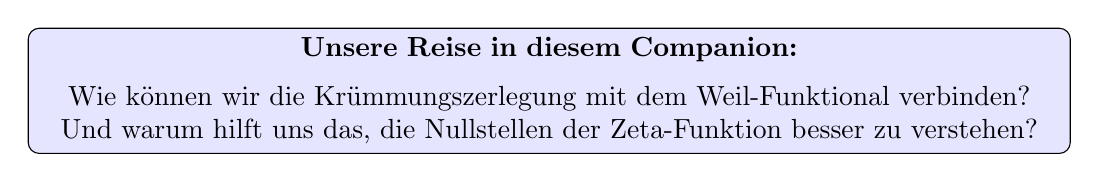
\begin{tikzpicture}
			\node[draw, fill=blue!10, rounded corners, text width=13cm, align=center] {
				\textbf{Unsere Reise in diesem Companion:}\\[0.2cm]
				Wie k\"onnen wir die Kr\"ummungszerlegung mit dem Weil-Funktional verbinden?\\
				Und warum hilft uns das, die Nullstellen der Zeta-Funktion besser zu verstehen?
			};
		\end{tikzpicture}
	\end{center}
	
	\subsection{Wiederholung: Was wissen wir bereits?}
	
	Aus dem ersten Companion wissen wir:
	\begin{itemize}
		\item Das Kr\"ummungsfeld $\Hxi(\sigma, t)$ misst die Kr\"ummung der
		Zeta-Funktion in Richtung der reellen Achse.
		\item Es l\"asst sich zerlegen in: $\Hxi = \Hlocal + \Hdual$.
		\item Der lokale Teil $\Hlocal$ besteht aus Beitr\"agen von Primzahlen und
		einem archimedischen Term.
		\item Auf der kritischen Linie $\sigma=\frac{1}{2}$ w\"achst $\Hlocal$ wie
		$(\log \kappa)^2$, wobei $\kappa$ der Primzahl-Grenzwert ist.
	\end{itemize}
	
	
	%% ============================================================
	%% TEIL 2: Weil-Funktional und Testfunktionen
	%% ============================================================
	
	\section{Das Weil-Funktional und Testfunktionen}\label{sec:weil_funktional}
	
	\subsection{Was ist das Weil-Funktional?}
	
	Das Weil-Funktional ist ein mathematisches Konstrukt, das von Andr\'e Weil
	eingef\"uhrt wurde. Es stellt eine tiefe Verbindung zwischen Primzahlen und
	den Nullstellen der Zeta-Funktion her.
	
	\begin{definition}[Weil-Funktional, vereinfacht]
		Das Weil-Funktional $W$ bildet eine Testfunktion $f$ auf eine reelle Zahl ab:
		\begin{equation}
			W(f * \check{f}) = \text{Konstante} + \text{Archimedischer Teil}
			+ \text{Primzahl-Teil} - \text{Nullstellen-Teil}
		\end{equation}
		Dabei ist $f * \check{f}$ die Faltung von $f$ mit ihrer Spiegelung $\check{f}$.
	\end{definition}
	
	\begin{remark}
		Die Bedeutung des Weil-Funktionals liegt in einem erstaunlichen Zusammenhang:
		
		Die Riemannsche Vermutung ist \"aquivalent zu:
		\begin{equation}
			W(f * \check{f}) \geq 0 \quad \text{f\"ur alle zul\"assigen Testfunktionen } f
		\end{equation}
		
		Die Riemannsche Vermutung, eine Aussage \"uber die Position von Nullstellen,
		l\"asst sich also in eine Aussage \"uber die \emph{Positivit\"at} eines
		Funktionals umformulieren!
	\end{remark}
	
	\subsection{Zul\"assige Testfunktionen}
	
	Nicht jede Funktion kann als Testfunktion f\"ur das Weil-Funktional verwendet werden.
	Eine Testfunktion muss besondere Eigenschaften haben.
	
	\begin{definition}[Zul\"assige Testfunktionen $\Sad$, vereinfacht]
		Eine Funktion $f$ geh\"ort zur Klasse $\Sad$ der zul\"assigen Testfunktionen, wenn:
		\begin{enumerate}
			\item $f$ und ihre Fourier-Transformierte schnell abfallen (Schwartz-Klasse).
			\item $f(0) = 0$ und $\hat{f}(0) = 0$ (Verschwinden am Ursprung).
		\end{enumerate}
	\end{definition}
	
	\begin{center}
		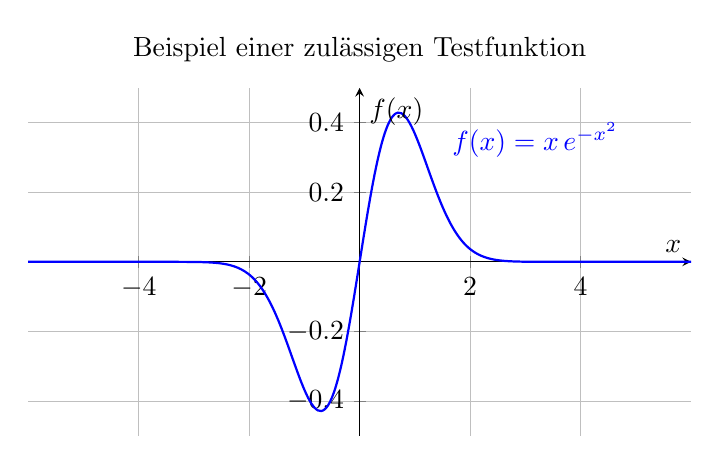
\begin{tikzpicture}
			\begin{axis}[
				title={Beispiel einer zul\"assigen Testfunktion},
				xlabel={$x$},
				ylabel={$f(x)$},
				xmin=-6, xmax=6,
				ymin=-0.5, ymax=0.5,
				xtick={-4,-2,0,2,4},
				ytick={-0.4,-0.2,0,0.2,0.4},
				grid=both,
				grid style={line width=.1pt, draw=gray!10},
				major grid style={line width=.2pt, draw=gray!50},
				axis lines=middle,
				width=10cm,
				height=6cm,
				]
				\addplot[thick, blue, smooth, domain=-6:6, samples=200] {x*exp(-x^2)};
				\node[blue, right] at (axis cs: 1.5, 0.35) {$f(x) = x\, e^{-x^2}$};
			\end{axis}
		\end{tikzpicture}
	\end{center}
	
	\begin{remark}
		Die Beispielfunktion $f(x) = x\, e^{-x^2}$ ist zul\"assig, weil:
		\begin{itemize}
			\item Sie ist antisymmetrisch: $f(-x) = -f(x)$.
			\item Sie verschwindet am Ursprung: $f(0) = 0$.
			\item Sie f\"allt schnell ab f\"ur gro\ss e $|x|$.
		\end{itemize}
	\end{remark}
	
	
	%% ============================================================
	%% TEIL 3: Konstruktion der Testfunktion
	%% ============================================================
	
	\section{Konstruktion einer speziellen Testfunktion}\label{sec:konstruktion}
	
	\subsection{Die Grundidee: Primzahlen als Bausteine}
	
	Wir konstruieren jetzt eine spezielle Testfunktion, die eine Verbindung zum
	Kr\"ummungsfeld herstellt. Die Grundidee ist faszinierend: Wir platzieren
	Gau\ss sche Glockenkurven an den Logarithmen der Primzahlen!
	
	\begin{center}
		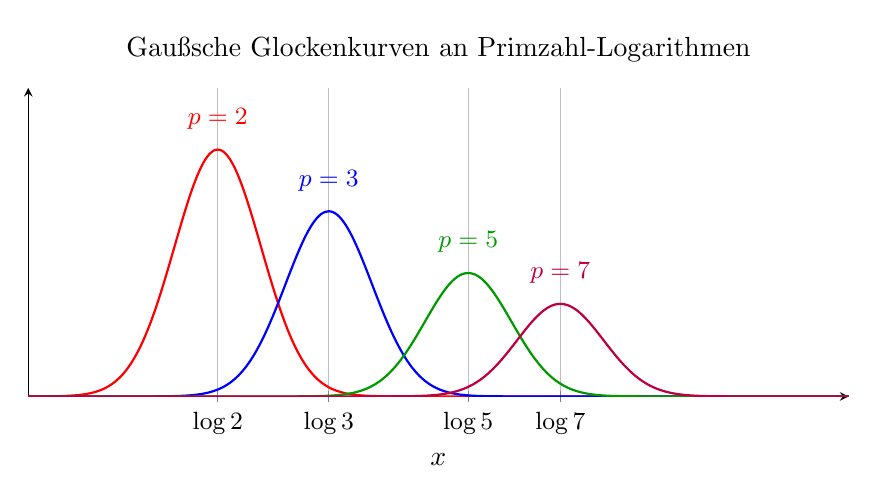
\begin{tikzpicture}
			\begin{axis}[
				title={Gau\ss sche Glockenkurven an Primzahl-Logarithmen},
				xlabel={$x$},
				ylabel={},
				xmin=0, xmax=3,
				ymin=0, ymax=10,
				xtick={0.693,1.099,1.609,1.946},
				xticklabels={$\log 2$,$\log 3$,$\log 5$,$\log 7$},
				x tick label style={font=\small},
				ytick=\empty,
				grid=major,
				axis lines=left,
				width=12cm,
				height=5.5cm,
				]
				\addplot[thick, red, smooth, domain=0:3, samples=200]
				{8*exp(-(x-0.693)^2/0.05)};
				\addplot[thick, blue, smooth, domain=0:3, samples=200]
				{6*exp(-(x-1.099)^2/0.05)};
				\addplot[thick, green!60!black, smooth, domain=0:3, samples=200]
				{4*exp(-(x-1.609)^2/0.05)};
				\addplot[thick, purple, smooth, domain=0:3, samples=200]
				{3*exp(-(x-1.946)^2/0.05)};
				\node[red, font=\small] at (axis cs: 0.693, 9) {$p=2$};
				\node[blue, font=\small] at (axis cs: 1.099, 7) {$p=3$};
				\node[green!60!black, font=\small] at (axis cs: 1.609, 5) {$p=5$};
				\node[purple, font=\small] at (axis cs: 1.946, 4) {$p=7$};
			\end{axis}
		\end{tikzpicture}
	\end{center}
	
	Jede Primzahl~$p$ erh\"alt eine Glockenkurve bei $x = \log p$, gewichtet mit
	einem Faktor, der von der Kr\"ummung $V_p(\sigma)$ abh\"angt. Kleine Primzahlen
	wie $p=2$ tragen st\"arker bei als gro\ss e.
	
	\subsection{Die Konstruktion in zwei Schritten}
	
	Wir bauen unsere Testfunktion $g^*_{\sigma,\varepsilon}$ in zwei Schritten:
	
	\begin{definition}[Konstruktion der Testfunktion]
		\begin{enumerate}
			\item \textbf{Schritt 1 --- Gau\ss sche Summe:}
			Wir definieren eine Funktion $\hat{f}_{\sigma,\varepsilon}$ als gewichtete
			Summe von Gau\ss schen Glockenkurven an den Logarithmen der Primzahlen:
			\begin{equation}
				\hat{f}_{\sigma,\varepsilon}(x)
				= \sum_{p \leq \kappa} c_{p,\sigma}\, \varphi_{\varepsilon}(x - \log p)
			\end{equation}
			Dabei ist $\varphi_{\varepsilon}(x) = \frac{1}{\varepsilon\sqrt{2\pi}}\,
			e^{-x^2/(2\varepsilon^2)}$ die Gau\ss sche Glockenkurve und $c_{p,\sigma}$
			ein spezielles Gewicht.
			
			\item \textbf{Schritt 2 --- Antisymmetrisierung:}
			Wir machen die Funktion antisymmetrisch, damit sie am Ursprung verschwindet:
			\begin{equation}
				\hat{g}^*_{\sigma,\varepsilon}(x)
				= \hat{f}_{\sigma,\varepsilon}(x) - \hat{f}_{\sigma,\varepsilon}(-x)
			\end{equation}
		\end{enumerate}
	\end{definition}
	
	Warum die Antisymmetrisierung? Das Weil-Funktional verlangt, dass $\hat{g}^*(0) = 0$.
	Da $\hat{f}$ \"uberall positiv ist, verschwindet $\hat{f}(0)$ nicht von alleine.
	Aber die Differenz $\hat{f}(x) - \hat{f}(-x)$ ist bei $x=0$ automatisch null!
	
	\begin{center}
		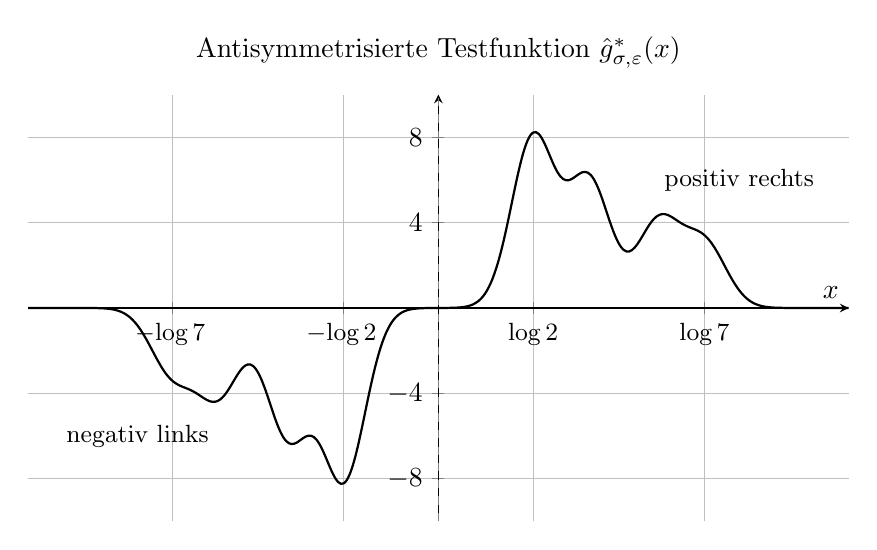
\begin{tikzpicture}
			\begin{axis}[
				title={Antisymmetrisierte Testfunktion $\hat{g}^*_{\sigma,\varepsilon}(x)$},
				xlabel={$x$},
				ylabel={},
				xmin=-3, xmax=3,
				ymin=-10, ymax=10,
				xtick={-1.946,-0.693,0,0.693,1.946},
				xticklabels={$\!-\!\log 7$,$\!-\!\log 2$,$0$,$\log 2$,$\log 7$},
				x tick label style={font=\small},
				ytick={-8,-4,0,4,8},
				grid=major,
				axis lines=middle,
				width=12cm,
				height=7cm,
				]
				% g* = f(x) - f(-x)
				\addplot[thick, black, smooth, domain=-3:3, samples=300]
				{8*exp(-(x-0.693)^2/0.05) + 6*exp(-(x-1.099)^2/0.05)
					+ 4*exp(-(x-1.609)^2/0.05) + 3*exp(-(x-1.946)^2/0.05)
					- 8*exp(-(x+0.693)^2/0.05) - 6*exp(-(x+1.099)^2/0.05)
					- 4*exp(-(x+1.609)^2/0.05) - 3*exp(-(x+1.946)^2/0.05)};
				\node[font=\small] at (axis cs: 2.2, 6) {positiv rechts};
				\node[font=\small] at (axis cs: -2.2, -6) {negativ links};
				\draw[dashed, gray] (axis cs: 0,-10) -- (axis cs: 0,10);
			\end{axis}
		\end{tikzpicture}
	\end{center}
	
	\begin{remark}
		Die Antisymmetrie $\hat{g}^*(-x) = -\hat{g}^*(x)$ ist der Schl\"ussel:
		Sie garantiert, dass die Funktion die Zul\"assigkeitsbedingung erf\"ullt,
		und sorgt gleichzeitig daf\"ur, dass der Konstantenterm im Weil-Funktional
		verschwindet.
	\end{remark}
	
	
	%% ============================================================
	%% TEIL 4: Verbindung zum Kr\"ummungsfeld
	%% ============================================================
	
	\section{Die Verbindung zum Kr\"ummungsfeld}\label{sec:verbindung}
	
	\subsection{Das Hauptresultat: Die Primzahl-Seite des Weil-Funktionals}
	
	Jetzt kommt der zentrale Schritt: Wenn wir unsere speziell konstruierte
	Testfunktion $g^*_{\sigma,\varepsilon}$ in das Weil-Funktional einsetzen,
	passiert etwas Bemerkenswertes.
	
	\begin{theorem}[Primzahl-Seiten-Identit\"at, vereinfacht]
		F\"ur die konstruierte Testfunktion $g^*_{\sigma,\varepsilon}$ gilt:
		\begin{equation}\label{eq:bridge}
			W(g^* * \check{g}^*)
			\;=\; \underbrace{Z(g^*)}_{\text{Nullstellen-Summe}}
			\;-\; \underbrace{\Hlocal(\sigma,\kappa)}_{\text{lokale Kr\"ummung}}
			\;+\; \underbrace{R(\sigma,\varepsilon,\kappa)}_{\text{kleiner Rest}}
		\end{equation}
		wobei der Rest $R$ f\"ur $\varepsilon \to 0$ verschwindet.
	\end{theorem}
	
	Was bedeutet diese Formel? Setzen wir sie in Worte um:
	
	\begin{center}
		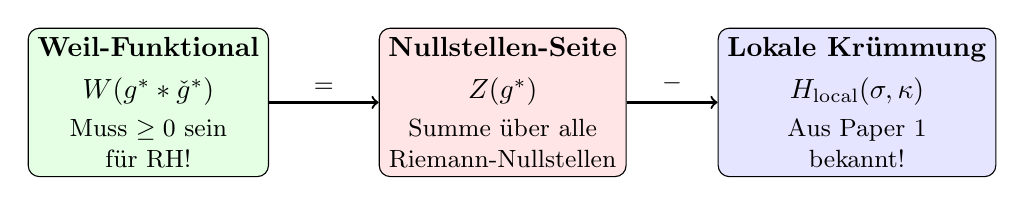
\begin{tikzpicture}
			% Drei Boxen
			\node[draw, fill=green!10, rounded corners, minimum width=3cm,
			minimum height=1.8cm, align=center] (weil) at (-4.5,0) {
				\textbf{Weil-Funktional}\\[3pt]
				$W(g^* * \check{g}^*)$\\[2pt]
				\small Muss $\geq 0$ sein\\[-1pt]
				\small f\"ur RH!
			};
			\node[draw, fill=red!10, rounded corners, minimum width=3cm,
			minimum height=1.8cm, align=center] (zero) at (0,0) {
				\textbf{Nullstellen-Seite}\\[3pt]
				$Z(g^*)$\\[2pt]
				\small Summe \"uber alle\\[-1pt]
				\small Riemann-Nullstellen
			};
			\node[draw, fill=blue!10, rounded corners, minimum width=3cm,
			minimum height=1.8cm, align=center] (local) at (4.5,0) {
				\textbf{Lokale Kr\"ummung}\\[3pt]
				$\Hlocal(\sigma,\kappa)$\\[2pt]
				\small Aus Paper~1\\[-1pt]
				\small bekannt!
			};
			\draw[->, thick] (weil) -- (zero) node[midway, above, font=\small] {$=$};
			\draw[->, thick] (zero) -- (local) node[midway, above, font=\small] {$-$};
		\end{tikzpicture}
	\end{center}
	
	\subsection{Warum ist das so wichtig?}
	
	Die Formel~\eqref{eq:bridge} ist die \emph{Br\"ucke} zwischen der
	Kr\"ummungszerlegung aus Paper~1 und dem Weil-Positivit\"ats-Rahmen.
	
	Erinnern wir uns: Die Riemannsche Vermutung ist \"aquivalent zu
	$W(g^* * \check{g}^*) \geq 0$. Die Formel sagt uns also:
	\[
	\underbrace{W \geq 0}_{\text{RH}}
	\quad\Longleftrightarrow\quad
	\underbrace{Z(g^*) \geq \Hlocal(\sigma,\kappa)}_{\text{Spektrale Ungleichung}}
	\]
	
	Die Frage, ob die Riemannsche Vermutung stimmt, wird f\"ur diese Testfunktion
	zur Frage: \"Uberwiegt die Nullstellen-Seite $Z(g^*)$ die lokale
	Kr\"ummung $\Hlocal$?
	
	\begin{remark}
		Drei Dinge aus Paper~1 gehen direkt ein:
		\begin{itemize}
			\item $\Hlocal \geq 0$ (immer positiv --- aus der Positivit\"at von $V_p$).
			\item Auf der kritischen Linie w\"achst $\Hlocal \sim 2(\log\kappa)^2$
			--- also muss auch $Z(g^*)$ mindestens so schnell wachsen!
			\item Der Konstantenterm verschwindet, weil $\hat{g}^*(0) = 0$
			(Antisymmetrie).
		\end{itemize}
	\end{remark}
	
	
	%% ============================================================
	%% TEIL 5: Renormalisierte Gewichte
	%% ============================================================
	
	\section{Renormalisierte Gewichte und die Diagonalenergie}\label{sec:renorm}
	
	\subsection{Das Problem der Skalenordnung}
	
	Auf der kritischen Linie $\sigma = \frac{1}{2}$ w\"achst $\Hlocal$ wie
	$2(\log\kappa)^2$. Das ist ein riesiger Beitrag! Um die feinere Struktur
	zu sehen, m\"ussen wir diesen dominanten Term ``herausrechnen''.
	
	\begin{definition}[Renormalisierte Kr\"ummung]
		Die \emph{renormalisierte} lokale Kr\"ummung ist:
		\begin{equation}
			\Hren(\tfrac{1}{2}, \kappa)
			\;:=\; \Hlocal(\tfrac{1}{2}, \kappa) - 2(\log\kappa)^2
		\end{equation}
		Sie misst, wie stark $\Hlocal$ vom dominanten Wachstumsterm abweicht.
	\end{definition}
	
	Stellt euch vor, ihr messt die H\"ohe von Bergen. Wenn alle Berge auf
	einem Plateau von 3000\,m stehen, ist es sinnvoller, die H\"ohe
	\emph{\"uber dem Plateau} zu messen, um die Unterschiede zwischen den
	Bergen zu sehen.
	
	\subsection{Renormalisierte Primzahl-Gewichte}
	
	F\"ur die feinere Analyse definieren wir ein neues Gewicht $\cren$,
	das die Abweichung von $V_p(\frac{1}{2})$ vom f\"uhrenden Term misst:
	
	\begin{definition}[Renormalisiertes Gewicht]
		\begin{equation}
			f_p \;:=\; V_p(\tfrac{1}{2}) - \frac{4(\log p)^2}{p}
			\;=\; \frac{4(\log p)^2(2p-1)}{p(p-1)^2}
		\end{equation}
		Das renormalisierte Gewicht ist dann $\cren := \sqrt{f_p}$.
	\end{definition}
	
	\begin{lemma}[Positivit\"at]
		F\"ur jede Primzahl $p \geq 2$ gilt $f_p > 0$, also ist $\cren$ wohldefiniert.
	\end{lemma}
	
	Das ist leicht zu sehen: Im Z\"ahler steht $2p - 1 > 0$ und im Nenner
	$p(p-1)^2 > 0$ f\"ur alle $p \geq 2$.
	
	Hier einige numerische Werte:
	
	\begin{center}
		\begin{tabular}{ccccc}
			\toprule
			$p$ & $V_p(\frac{1}{2})$ & $\frac{4(\log p)^2}{p}$ & $f_p = (\cren)^2$ & $\cren$ \\
			\midrule
			2  & 3{,}844 & 0{,}961 & 2{,}883 & 1{,}698 \\
			3  & 3{,}621 & 1{,}609 & 2{,}012 & 1{,}418 \\
			5  & 3{,}238 & 2{,}072 & 1{,}166 & 1{,}080 \\
			7  & 2{,}945 & 2{,}164 & 0{,}781 & 0{,}884 \\
			11 & 2{,}530 & 2{,}091 & 0{,}439 & 0{,}663 \\
			\bottomrule
		\end{tabular}
	\end{center}
	
	Man sieht: Die Gewichte $f_p$ werden f\"ur gr\"o\ss ere Primzahlen immer kleiner.
	Das f\"uhrt zu einer wichtigen Eigenschaft:
	
	\subsection{Die Diagonalenergie $D$}
	
	\begin{definition}[Diagonalenergie]
		Die \emph{Diagonalenergie} ist die Summe aller renormalisierten Gewichte:
		\begin{equation}
			D \;:=\; \sum_p (\cren)^2 \;=\; \sum_p f_p
			\;=\; \sum_p \frac{4(\log p)^2(2p-1)}{p(p-1)^2}
		\end{equation}
	\end{definition}
	
	\begin{lemma}[Konvergenz der Diagonalenergie]
		Die Reihe $D = \sum_p f_p$ konvergiert. Numerisch: $D \approx 9{,}471$.
	\end{lemma}
	
	Die Konvergenz folgt daraus, dass f\"ur gro\ss e Primzahlen
	$f_p \sim 8(\log p)^2/p^2$ gilt, und die Reihe $\sum_n (\log n)^2/n^2$
	ist konvergent.
	
	\begin{remark}
		Die Diagonalenergie $D \approx 9{,}471$ ist eine feste arithmetische Konstante
		--- sie h\"angt nur von den Primzahlen ab, nicht von der Riemannschen Vermutung
		oder irgendwelchen Hypothesen. Sie spielt eine zentrale Rolle als
		\emph{Ma\ss stab} f\"ur die Primzahl-Seite der Br\"uckenformel.
	\end{remark}
	
	
	%% ============================================================
	%% TEIL 6: S\"agezahn und Mertens-Konstante
	%% ============================================================
	
	\section{Die S\"agezahn-Struktur und die Mertens-Konstante}\label{sec:saegezahn}
	
	\subsection{Springen und Fallen}
	
	Die renormalisierte Kr\"ummung $\Hren(\frac{1}{2}, \kappa)$ zeigt ein
	faszinierendes Verhalten, wenn man $\kappa$ ver\"andert:
	
	\begin{itemize}
		\item Bei jeder neuen Primzahl $p \leq \kappa$ \emph{springt} $\Hren$
		um $f_p$ nach oben.
		\item Zwischen aufeinanderfolgenden Primzahlen \emph{f\"allt} $\Hren$
		kontinuierlich, weil $2(\log\kappa)^2$ w\"achst, ohne dass neue
		Primterme hinzukommen.
	\end{itemize}
	
	Das ergibt ein \emph{S\"agezahnmuster}:
	
	\begin{center}
		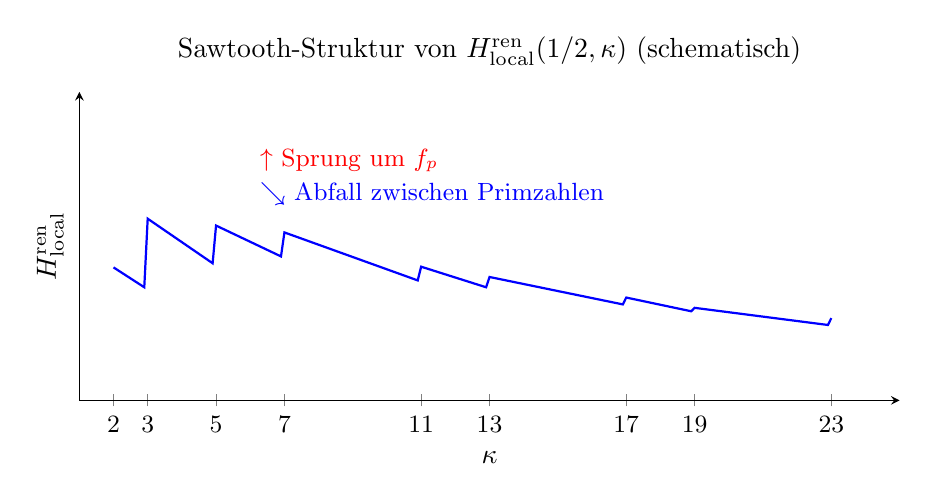
\begin{tikzpicture}
			\begin{axis}[
				title={Sawtooth-Struktur von $\Hren(1/2, \kappa)$ (schematisch)},
				xlabel={$\kappa$},
				ylabel={$\Hren$},
				xmin=1, xmax=25,
				ymin=-1, ymax=8,
				xtick={2,3,5,7,11,13,17,19,23},
				xticklabels={$2$,$3$,$5$,$7$,$11$,$13$,$17$,$19$,$23$},
				x tick label style={font=\small},
				ytick=\empty,
				axis lines=left,
				width=12cm,
				height=5.5cm,
				]
				\addplot[thick, blue, mark=none] coordinates {
					(2,2.88) (2.9,2.3)
					(3,4.3) (4.9,3.0)
					(5,4.1) (6.9,3.2)
					(7,3.9) (10.9,2.5)
					(11,2.9) (12.9,2.3)
					(13,2.6) (16.9,1.8)
					(17,2.0) (18.9,1.6)
					(19,1.7) (22.9,1.2)
					(23,1.4)
				};
				\node[red, font=\small, right] at (axis cs: 6, 6) {$\uparrow$ Sprung um $f_p$};
				\node[blue, font=\small, right] at (axis cs: 6, 5) {$\searrow$ Abfall zwischen Primzahlen};
			\end{axis}
		\end{tikzpicture}
	\end{center}
	
	\subsection{Die Mertens-Konstante}
	
	Das durchschnittliche Verhalten dieses S\"agezahns wird von der
	\emph{Mertens-Konstante} gesteuert:
	\[
	\gamma_M = \gamma + \sum_p \Bigl[\log\bigl(1-\tfrac{1}{p}\bigr) + \tfrac{1}{p}\Bigr]
	\approx 0{,}2615
	\]
	wobei $\gamma \approx 0{,}5772$ die Euler--Mascheroni-Konstante ist.
	
	\begin{remark}
		Die Mertens-Konstante $\gamma_M$ taucht auch beim ersten Li-Koeffizienten auf:
		\[
		\lambda_1 = 1 + \tfrac{\gamma}{2} - \log 2 - \tfrac{\log\pi}{2}
		\approx 0{,}0231
		\]
		Das zeigt, wie tief die Verbindung zwischen Primzahl-Summen und der
		Zeta-Funktion reicht.
	\end{remark}
	
	
	%% ============================================================
	%% TEIL 7: Numerischer Vergleich
	%% ============================================================
	
	\section{Numerischer Vergleich: Nullstellen vs.\ Kr\"ummung}\label{sec:numerik}
	
	\subsection{Die entscheidende Frage}
	
	Erinnern wir uns: Die Riemannsche Vermutung f\"ur unsere Testfunktion
	ist gleichbedeutend mit $Z(g^*) \geq \Hlocal$, also:
	
	\emph{\"Uberwiegt die Nullstellen-Seite die lokale Kr\"ummung?}
	
	Um das zu pr\"ufen, vergleichen wir die renormalisierten Gr\"o\ss en auf
	einem Gitter von $\kappa$-Werten:
	
	\begin{center}
		\begin{tabular}{ccccc}
			\toprule
			$\kappa$ & $\Zren$ & $\Hren$ & $\Zren - \Hren$ & $\Zren \geq \Hren$\,? \\
			\midrule
			10   & 4{,}888 & 3{,}044 & $+1{,}844$ & \checkmark \\
			20   & 3{,}782 & 4{,}770 & $-0{,}988$ & $\times$ \\
			29   & 5{,}520 & 3{,}588 & $+1{,}931$ & \checkmark \\
			50   & 5{,}693 & 2{,}881 & $+2{,}812$ & \checkmark \\
			100  & 5{,}311 & 1{,}562 & $+3{,}748$ & \checkmark \\
			200  & 5{,}102 & 2{,}355 & $+2{,}747$ & \checkmark \\
			500  & 5{,}156 & 1{,}101 & $+4{,}056$ & \checkmark \\
			1000 & 4{,}289 & 0{,}426 & $+3{,}863$ & \checkmark \\
			\bottomrule
		\end{tabular}
	\end{center}
	
	\subsection{Was sehen wir?}
	
	\begin{itemize}
		\item Bei \textbf{sieben von acht} Testpunkten gilt $\Zren \geq \Hren$
		--- die Nullstellen-Seite \"uberwiegt!
		\item Die einzige Ausnahme ist $\kappa = 20$, wo $\Zren - \Hren = -0{,}988$.
		Das liegt an der S\"agezahn-Struktur: Direkt nach dem Primzahl-Sprung bei
		$p = 19$ ist $\Hren$ besonders hoch.
		\item Das Verh\"altnis $\Zren / \Hren$ \emph{w\"achst} mit $\kappa$:
		von $1{,}5$ bei $\kappa = 29$ auf \"uber $10$ bei $\kappa = 1000$.
	\end{itemize}
	
	\begin{center}
		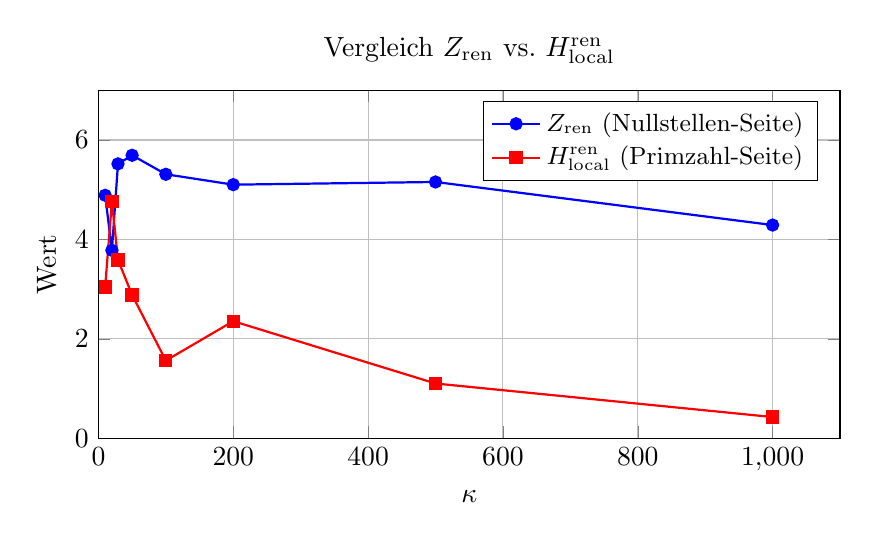
\begin{tikzpicture}
			\begin{axis}[
				title={Vergleich $\Zren$ vs.\ $\Hren$},
				xlabel={$\kappa$},
				ylabel={Wert},
				xmin=0, xmax=1100,
				ymin=0, ymax=7,
				legend pos=north east,
				legend style={font=\small},
				grid=major,
				width=11cm,
				height=6cm,
				]
				\addplot[thick, blue, mark=*, mark size=2pt] coordinates {
					(10,4.888) (20,3.782) (29,5.520) (50,5.693)
					(100,5.311) (200,5.102) (500,5.156) (1000,4.289)
				};
				\addlegendentry{$\Zren$ (Nullstellen-Seite)}
				\addplot[thick, red, mark=square*, mark size=2pt] coordinates {
					(10,3.044) (20,4.770) (29,3.588) (50,2.881)
					(100,1.562) (200,2.355) (500,1.101) (1000,0.426)
				};
				\addlegendentry{$\Hren$ (Primzahl-Seite)}
			\end{axis}
		\end{tikzpicture}
	\end{center}
	
	\begin{remark}
		Diese numerischen Befunde sind \emph{konsistent} mit der Riemannschen
		Vermutung, aber sie \emph{beweisen} sie nicht. Ein Beweis m\"usste
		zeigen, dass die Ungleichung f\"ur \emph{alle} $\kappa$ gilt, nicht
		nur f\"ur acht Testpunkte.
	\end{remark}
	
	\subsection{Die Br\"uckenkonstante $D/2\pi$}
	
	Unter der Annahme, dass die ``Nebendiagonale'' (die Kreuzterme mit
	$p \neq q$) vernachl\"assigbar ist, ergibt sich f\"ur die
	Nullstellen-Seite die formale Asymptotik
	$Z(g^*) \sim D \cdot \log\kappa \cdot \log\log\kappa$.
	Das f\"uhrt zu einer nat\"urlichen Br\"uckenkonstante:
	\[
	\frac{D}{2\pi} \approx \frac{9{,}471}{6{,}283} \approx 1{,}507
	\]
	Diese Konstante misst das Verh\"altnis der Primzahl-Energie $D$
	zur archimedischen Normierung $2\pi$ der Nullstellen-Dichte
	$N(T) \sim T \log T / (2\pi)$.
	
	\begin{remark}
		Wichtig: Die Br\"uckenkonstante $D/2\pi$ h\"angt nur von der
		\emph{Gesamtdichte} der Nullstellen ab, nicht von ihrer
		Paar-Korrelation. Sie hat nichts mit der GUE-Vermutung zu tun!
	\end{remark}
	
	
	%% ============================================================
	%% TEIL 8: Offene Fragen
	%% ============================================================
	
	\section{Offene Fragen und Bedeutung f\"ur die Riemannsche Vermutung}\label{sec:offen}
	
	\subsection{Was ist bewiesen, was ist offen?}
	
	Fassen wir den Status zusammen:
	
	\begin{center}
		\begin{tabular}{p{7cm}cc}
			\toprule
			\textbf{Aussage} & \textbf{Status} \\
			\midrule
			$g^*_{\sigma,\varepsilon}$ ist zul\"assige Testfunktion & \textbf{Bewiesen} \\
			$\cren = \sqrt{f_p} > 0$ f\"ur alle Primzahlen & \textbf{Bewiesen} \\
			$D = \sum_p f_p$ konvergiert ($\approx 9{,}471$) & \textbf{Bewiesen} \\
			Primzahl-Seiten-Identit\"at (Formel~\ref{eq:bridge}) & Bedingt \\
			$\Zren \geq \Hren$ auf Testgitter (7/8 Punkte) & Numerisch \\
			$Z(g^*) \geq \Hlocal$ f\"ur \emph{alle} $\kappa$ & \textbf{Offen} \\
			\bottomrule
		\end{tabular}
	\end{center}
	
	\subsection{Die zwei offenen Probleme}
	
	Zwei Fragen trennen die aktuelle Konstruktion von einem vollst\"andigen
	Beweis der Weil-Positivit\"at f\"ur diese Testfunktionen-Familie:
	
	\begin{center}
		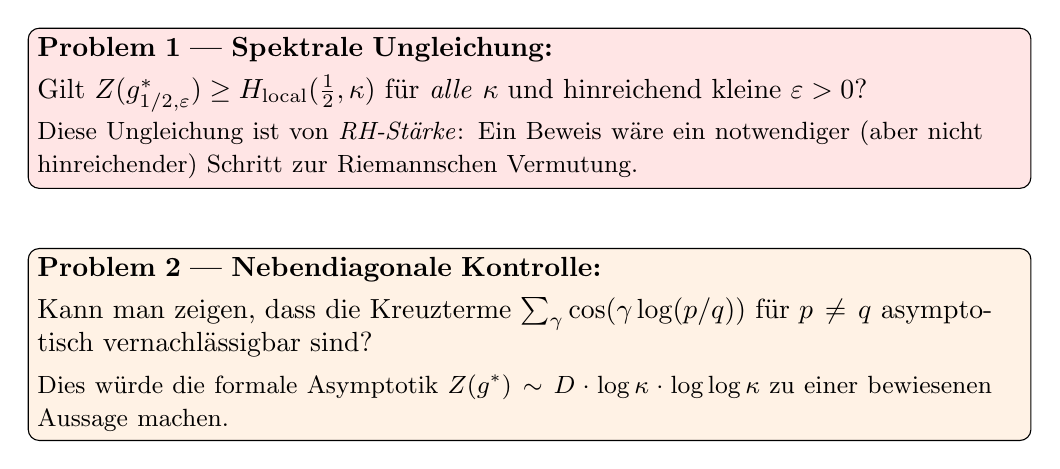
\begin{tikzpicture}
			\node[draw, fill=red!10, rounded corners, text width=12.5cm, align=left]
			at (0,3) {
				\textbf{Problem 1 --- Spektrale Ungleichung:}\\[3pt]
				Gilt $Z(g^*_{1/2,\varepsilon}) \geq \Hlocal(\frac{1}{2}, \kappa)$
				f\"ur \emph{alle} $\kappa$ und hinreichend kleine $\varepsilon > 0$?\\[3pt]
				\small Diese Ungleichung ist von \emph{RH-St\"arke}: Ein Beweis w\"are ein
				notwendiger (aber nicht hinreichender) Schritt zur Riemannschen Vermutung.
			};
			\node[draw, fill=orange!10, rounded corners, text width=12.5cm, align=left]
			at (0,0) {
				\textbf{Problem 2 --- Nebendiagonale Kontrolle:}\\[3pt]
				Kann man zeigen, dass die Kreuzterme $\sum_\gamma \cos(\gamma \log(p/q))$
				f\"ur $p \neq q$ asymptotisch vernachl\"assigbar sind?\\[3pt]
				\small Dies w\"urde die formale Asymptotik
				$Z(g^*) \sim D \cdot \log\kappa \cdot \log\log\kappa$
				zu einer bewiesenen Aussage machen.
			};
		\end{tikzpicture}
	\end{center}
	
	\subsection{Der Weg vorw\"arts}
	
	\begin{center}
		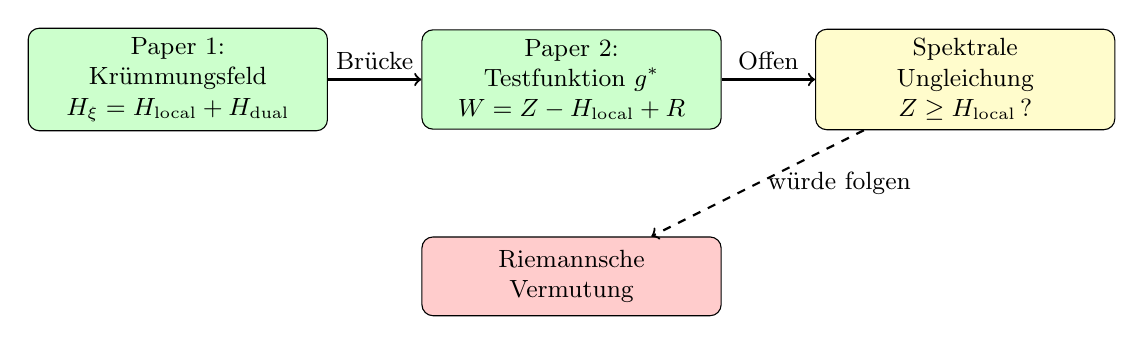
\begin{tikzpicture}[node distance=1.6cm, every node/.style={font=\small}]
			\node[draw, fill=green!20, rounded corners, minimum width=3.8cm,
			minimum height=1cm, align=center] (p1) at (0,0)
			{Paper 1:\\Kr\"ummungsfeld\\$\Hxi = \Hlocal + \Hdual$};
			\node[draw, fill=green!20, rounded corners, minimum width=3.8cm,
			minimum height=1cm, align=center] (p2) at (5,0)
			{Paper 2:\\Testfunktion $g^*$\\$W = Z - \Hlocal + R$};
			\node[draw, fill=yellow!20, rounded corners, minimum width=3.8cm,
			minimum height=1cm, align=center] (sp) at (10,0)
			{Spektrale\\Ungleichung\\$Z \geq \Hlocal$\,?};
			\node[draw, fill=red!20, rounded corners, minimum width=3.8cm,
			minimum height=1cm, align=center] (rh) at (5,-2.5)
			{Riemannsche\\Vermutung};
			\draw[->, thick] (p1) -- (p2) node[midway, above] {Br\"ucke};
			\draw[->, thick] (p2) -- (sp) node[midway, above] {Offen};
			\draw[->, thick, dashed] (sp) -- (rh) node[midway, right] {w\"urde folgen};
		\end{tikzpicture}
	\end{center}
	
	
	%% ============================================================
	%% TEIL 9: Zusammenfassung
	%% ============================================================
	
	\section{Zusammenfassung}\label{sec:zusammenfassung}
	
	In diesem Companion haben wir gesehen:
	
	\begin{enumerate}
		\item \textbf{Das Weil-Funktional} reformuliert die Riemannsche Vermutung als
		Positivit\"ats-Aussage: $W(f * \check{f}) \geq 0$ f\"ur alle zul\"assigen $f$.
		
		\item \textbf{Die Testfunktion $g^*$} wird explizit aus Primzahlen gebaut:
		Gau\ss sche Glockenkurven bei $\log p$, antisymmetrisiert.
		
		\item \textbf{Die Br\"uckenformel} verbindet Kr\"ummung und Weil-Funktional:
		$W = Z - \Hlocal + R$, wobei $\Hlocal$ genau die lokale Kr\"ummung aus
		Paper~1 ist.
		
		\item \textbf{Die Diagonalenergie} $D \approx 9{,}471$ konvergiert und ist
		eine feste arithmetische Konstante.
		
		\item \textbf{Numerisch} \"uberwiegt die Nullstellen-Seite die
		Kr\"ummungs-Seite bei fast allen getesteten $\kappa$-Werten.
		
		\item \textbf{Offen} bleibt, ob $Z(g^*) \geq \Hlocal$ f\"ur \emph{alle}
		$\kappa$ gilt --- das ist die spektrale Ungleichung, die zur
		Riemannschen Vermutung f\"uhren w\"urde.
	\end{enumerate}
	
	\begin{center}
		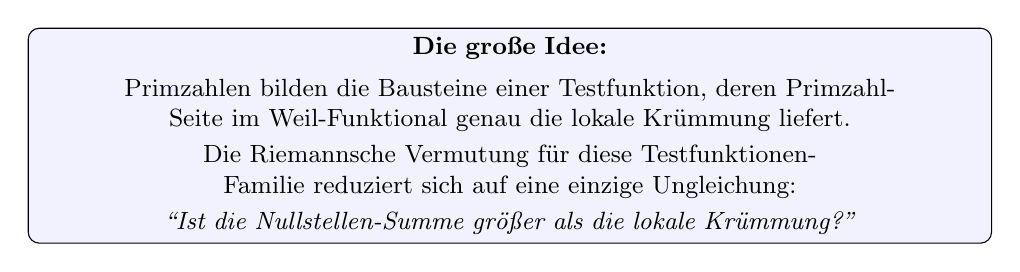
\begin{tikzpicture}
			\node[draw, fill=blue!5, rounded corners, text width=12cm, align=center,
			font=\small] {
				\textbf{Die gro\ss e Idee:}\\[4pt]
				Primzahlen bilden die Bausteine einer Testfunktion, deren
				Primzahl-Seite im Weil-Funktional genau die lokale Kr\"ummung liefert.\\[2pt]
				Die Riemannsche Vermutung f\"ur diese Testfunktionen-Familie
				reduziert sich auf eine einzige Ungleichung:\\[2pt]
				\emph{``Ist die Nullstellen-Summe gr\"o\ss er als die lokale Kr\"ummung?''}
			};
		\end{tikzpicture}
	\end{center}
	
	
	%% ============================================================
	%% ANHANG: Glossar
	%% ============================================================
	
	\newpage
	\section*{Glossar}
	
	\begin{description}
		\item[Antisymmetrisierung]
		Aus einer Funktion $f$ wird $g(x) = f(x) - f(-x)$ gebildet.
		Dadurch gilt automatisch $g(0) = 0$.
		
		\item[Archimedischer Term]
		Der Beitrag der ``unendlichen Stelle'' (der reellen Zahlen selbst,
		im Gegensatz zu den Primzahlen als ``endliche Stellen'').
		Im Kr\"ummungsfeld: $\psi_1(\sigma)$.
		
		\item[Diagonalenergie $D$]
		Die Summe $D = \sum_p f_p \approx 9{,}471$, wobei $f_p$ das
		renormalisierte Gewicht jeder Primzahl ist. Konvergiert, weil
		$f_p \sim 8(\log p)^2/p^2$ f\"ur gro\ss e $p$.
		
		\item[Faltung $f * g$]
		Die Funktion $(f * g)(x) = \int f(x-t)\, g(t)\, dt$.
		Im Weil-Funktional tritt $f * \check{f}$ auf, wobei
		$\check{f}(x) = \overline{f(-x)}$.
		
		\item[Mertens-Konstante $\gamma_M$]
		$\gamma_M \approx 0{,}2615$. Steuert das durchschnittliche
		Verhalten von Primzahl-Summen der Form $\sum_{p \leq x} 1/p$.
		
		\item[Renormalisierung]
		Herausrechnen des dominanten Wachstumsterms $2(\log\kappa)^2$
		aus $\Hlocal$, um die feinere Struktur sichtbar zu machen.
		
		\item[Schwartz-Klasse]
		Funktionen, die zusammen mit all ihren Ableitungen schneller
		als jede Potenz von $1/|x|$ abfallen.
		
		\item[Spektrale Ungleichung]
		Die offene Frage $Z(g^*) \geq \Hlocal$ --- gleichbedeutend mit
		$W \geq 0$ f\"ur die konstruierte Testfunktion.
		
		\item[Weil-Funktional $W$]
		Ein Funktional auf Testfunktionen, dessen Positivit\"at
		\"aquivalent zur Riemannschen Vermutung ist (Lagarias 1999,
		nach Weil 1952).
	\end{description}
	
\end{document}